\documentclass[article]{jss}
\usepackage{amsfonts,thumbpdf}

\newtheorem{lemma}{Lemma}
\newtheorem{theorem}{Theorem}
\newtheorem{corollary}{Corollary}
\newtheorem{example}{Example}
\newtheorem{proposition}{Proposition}
\newtheorem{definition}{Definition}
\newtheorem{conjecture}{Conjecture}
\newtheorem{assumption}{Assumption}
\def\logit{\mathop{\rm logit\,}\nolimits}
\def\midd{\mathop{\,|\,}\nolimits}
\def\defn{{\stackrel{\rm def}{=}}}
\def\eqdistn{{\stackrel{\cal D}{=}}}
\newcommand{\bea}{\begin{eqnarray}}
\newcommand{\eea}{\end{eqnarray}}
\newcommand{\beaa}{\begin{eqnarray*}}
\newcommand{\eeaa}{\end{eqnarray*}}
\newcommand{\qed}{{\rule{2mm}{2mm}}}
\newcommand{\en}{{\rule{.75em}{0cm}}}
\newcommand{\svskip}{\vspace{.125in}}
\newcommand{\mvskip}{\vspace{.25in}}
\newcommand{\lvskip}{\vspace{.5in}}
\newcommand{\R}{\mathbb{R}}

\def\vec#1{\mathchoice{\mbox{\boldmath$\displaystyle\bf#1$}}
{\mbox{\boldmath$\textstyle\bf#1$}}
{\mbox{\boldmath$\scriptstyle\bf#1$}}
{\mbox{\boldmath$\scriptscriptstyle\bf#1$}}}

\title{\pkg{ergmuserterms}: A Template Package}
\Plaintitle{ergmuserterms: A Template Package}
\Shorttitle{\pkg{ergmuserterms}: A Template Package}

\author{
  David R.\ Hunter \\ Penn State University \And
  Steven M.\ Goodreau \\ University of Washington \And
  Mark S.\ Handcock \\ University of Washington 
}
\Plainauthor{David R. Hunter, Steven M. Goodreau, Mark S. Handcock}

\Abstract { 
Abstract here
}
\Keywords{
exponential-family random graph model, Markov chain Monte Carlo, maximum likelihood estimation, p-star model}

%\Volume{}
%\Issue{}
%\Month{}
%\Year{}
%\Submitdate{}
%\Acceptdate{}

\Address{
David R.\ Hunter \\
Department of Statistics \\
Pennsylvania State University \\
University Park, PA 16802, United States of America\\
E-mail: \email{dhunter@stat.psu.edu} \\
URL: \url{http://www.stat.psu.edu/~dhunter/}
}

\begin{document}

\section{Introduction}
\label{introduction}

At the core of the \pkg{ergm} package \citep{ergm} 
for \proglang{R} \citep{r2010}
is a sophisticated 
Markov chain Monte Carlo engine for simulating random networks.  
As explained by \citet{ergmjss}, simulating a Markov chain on a
set of networks 
whose stationary distribution is given
by the exponential-family random graph model
\bea\label{ergm}
P_{\vec\theta_0} (\vec Y = \vec y) = 
\frac{ \exp\{ \vec \theta_0^\top  \vec g(\vec y) \} }
{ \kappa(\vec\theta)}
\eea
is vitally important not only for simulation but also for estimation.
In equation (\ref{ergm}), $\vec\theta_0\in \R^p$ is a fixed parameter vector,
$\vec g(\vec y)$ is a user-defined $p$-vector of statistics on the
network $\vec y$ assumed to come from some set ${\cal Y}$ of networks, and 
\bea\label{kappa}
\kappa(\vec\theta) = \sum_{\vec z \in {\cal Y}} \exp\{ \vec \theta_0^\top  \vec g(\vec z) \}
\eea
is the normalizing constant.

The MCMC scheme implemented in \pkg{ergm} is called a Metropolis-Hastings
algorithm.  In general terms, such an algorithm proceeds from step $t$ to step $t+1$,
from one network $\vec y^t$ to the next, by (a) selecting a candidate
for the next network $\vec y^{t+1}$, (b) computing a {\em Hastings ratio} based on
$\vec y^t$ and the candidate network, and (c) deciding whether $\vec y^{t+1}$
should be set to the candidate network or, alternatively, whether to stay put 
for another iteration and set $\vec y^{t+1}=\vec y^t$.
The selection (a) is done so that any possible network, say $\vec x$, has probability
$q(\vec x, \vec y^t)$ of being selected, where $q$ is some probability function known 
to the user.  (The $q$ function can and, in general, does put probability zero on
some values of $\vec x$, depending on the value of $\vec y^t$.)  
The Hastings ratio (b) is equal to
\begin{equation}\label{hastings}
\frac{P_{\vec\theta_0} (\vec Y=\vec y^t)}{P_{\vec\theta_0} (\vec Y=\vec x)}
\frac{q (\vec y^t, \vec x)}{q (\vec x, \vec y^t)},
\end{equation}
where $\vec x$ is the candidate network selected in (a).  Finally, (c) is done by selecting 
a real number, say $u$, uniformly from the unit interval (0,1) and comparing $u$ with
the Hastings ratio.  Then
\[
\vec y^{t+1} = \cases{\vec x & if $u \le \mbox{Hastings ratio}$; \cr
\vec y^t & if $u>\mbox {Hastings ratio}$.}
\]
In particular, note that if the Hastings ratio is greater than one, the candidate $\vec x$ is 
always accepted as the value for $\vec y^{t+1}$.

In \pkg{ergm}, there are different possible choices of the probability distribution $q(\vec x, \vec y_{t})$
used to select $\vec x$, but for the most part they all limit the possible choices of $\vec x$
to those that differ from $\vec y^t$ by exactly one edge indicator;  in other words, $\vec x$
involves a single edge toggle of $\vec y^t$.  Suppose that $\vec x$ is identical to $\vec y^t$
in all except the $(i,j)$ entry.  Notationally, we would write $x_{ij}=1-y_{ij}^t$ but
$\vec x_{ij}^c=\vec (y^t_{ij})^c$, where $\vec x_{ij}^c$ denotes the entire network $\vec x$ 
{\em except for} the $(i,j)$ entry.  In this case, by substituting Equation~(\ref{ergm}) into 
Expression~(\ref{hastings}), we see that the Hastings ratio may be simplified to
\begin{equation}\label{hastings2}
\frac{q (\vec y^t, \vec x)}{q (\vec x, \vec y^t)} \exp\{\pm \vec\theta_0^\top \delta (\vec y^t)_{ij} \},
\end{equation}
where 
\begin{equation}\label{changestats}
\delta (\vec y)_{ij} \stackrel{\rm def}{=} \vec g(\vec y_{ij}^+) - \vec g(\vec y_{ij}^-)
\end{equation}
denotes the {\em vector of change statistics}, found by subtracting the two vectors of
$\vec g$-statistics evaluated at the networks formed by leaving all of $\vec y$ unchanged
except for the $(i,j)$ entry, which is set to 1 in $\vec y_{ij}^+$ and 0 in $\vec y_{ij}^0$.
The sign of the $\vec\theta_0^\top \delta (\vec y^t)_{ij}$ term
in~(\ref{hastings2}) depends on the value
of $y_{ij}^t$:  If $y_{ij}^t=1$, then the term gets a plus sign; otherwise it gets a minus.

The key conclusion of all of the above development is that the calculation of 
change statistic vectors is of vital importance to the running of both the simulation and
the estimation routines in the \pkg{ergm}.   While the \pkg{ergm} package itself provides
a large library of possible change-statistic calculation routines \citep{ergmtermsjss}, 
individual users sometimes wish to write their own code for calculating change 
statistics for specialized network statistics so that the \pkg{ergm} estimation routines
can use it.  This article describes an \proglang{R} package called 
\pkg{ergmuserterms} that is designed to make this process as straightforward as possible.
It also explains some of the internal workings of the \pkg{ergm} package that will
help users develop their own network change statistic code.

In Section~\ref{syntax}, we discuss the unique syntax implemented in the \pkg{ergm}
package and explain why it was necessary to extend the existing formula-based
syntax (as used, say, by the \code{lm} and \code{glm} functions in \proglang{R})
to handle models that look like Equation~\ref{ergm}.  

\section[Syntax for a call to the ergm function]{Syntax for a call to the \code{ergm} function}
\label{syntax}

A traditional generalized linear model, as explained in the classic book by
\citet{mccullaghnelder1989}, consists of a specification of the probabilistic dependence
of some {\em response} variable, usually denoted $Y$, on some
function of a linear combination of some other {\em predictor} variables,
usually denoted $X$.  The distribution of $Y$ is generally a member of some
known exponential family; 
In its simplest form (ignoring any dispersion parameters), we may write the
density or mass function of $Y$, which depends on some
parameter vector $\vec\phi$, as
\[
f_Y(y) = \exp\{ \vec a(y)^\top \vec b(\vec\phi) - c(\vec\phi) \}.
\]
Standard exponential family theory \citep[for example, see][]{brown1986fse}
reveals that $E(Y) = (\partial / \partial\vec\phi) c(\vec\phi)$.
In a generalized linear model, we presume that
\[
E(Y) = \mbox{link}(\vec X^\top \vec\beta)
\]
for some ``link'' function.  Implicit in this formulation is the
fact that $\vec X$ in considered a fixed quantity, independent of $Y$;
indeed $\vec X$ is often referred to as the {\em independent} variable.
(Even when $\vec X$ is considered random, we typically specify a generalized
linear model for the {\em conditional} distribution of $Y$ given $\vec X$, so
that $\vec X$ may be considered constant in this context.)

In contrast, model~(\ref{ergm}) does not in general conform to the above 
specifications of a generalized linear model.  While it is true that the distribution of
the network $\vec Y$---the ``response''---is expressed in exponential family
form, there is no way to specify some fixed $\vec X$ and some link function so that
$E(\vec Y)= \mbox{link}(\vec X^\top \vec\beta)$.  Essentially, this is because
an ERGM involves an inherent auto-dependence between the ``response'' and 
any traditional notion of the ``predictors''.  

In addition, there is 
no closed-form expression for the likelihood function in an ERGM that
can be easily evaluated.  Equation~\ref{ergm} is generally impossible 
to use for the purposes of calculation due to the fact that
the $\kappa$ function of~\ref{kappa}) involves an enormous number
of summands for even simple networks.  Thus, even the estimation methods
necessitated by maximum likelihood estimation for an ERGM differ from those
used by a generalized linear model.  In the former case, we rely on MCMC
sampling to generate an approximation to the likelihood, whereas in the
latter the likelihood may be evaluated, and thus maximized, directly.

Because an ERGM is not a generalized linear model,
it is not possible to use exactly the same \proglang{R} syntax used for
\code{glm} calls  in order to specify a call to \code{ergm}.  
A call to \code{glm} might look like this:
\begin{CodeChunk}
\begin{CodeInput} 
R> glm ( response ~ predictor1 + predictor2 + predictor3, link = binomial)
\end{CodeInput}
\end{CodeChunk}
Since there is no way to define \code{predictorX} for a general ERGM,
we instead 

{\bf Remark:\ }
For certain choices of the vector $\vec g(\vec y)$ of graph statistics, the resulting
model~(\ref{ergm}) actually implies that all of the individual $y_{ij}$ edge indicators
are jointly independent.  In these cases, model~(\ref{ergm}) is actually equivalent
to a logistic regression model, which {\em is} a generalized linear model.
See Section~3 of \citet{HunGoodHan08} for more details on these so-called
independence models.
{\em Is there a better reference than this?}

\vspace{2ex}
\hrule

This section will:
\begin{itemize}
\item Argue that an ergm is not a glm because of its inherent auto-dependence.
Reasons include:  No closed-form expression for the likelihood (hence a dependence
on MCMC); no fixed matrix of predictors
\item Explain the syntax of an ergm formula (briefly; mostly, we can simply cite
\citet{ergmtermsjss}).
\end{itemize}

\section[Network storage in ergm]{Network storage in \pkg{ergm}}

A network with $n$ nodes is
internally represented in \pkg{ergm} as a set of $2n$ edgelists, 
$n$ for ``in-edges'' and $n$ for ``out-edges''.  If the directed edge $(3,5)$ exists in the network,
then we call 3 the ``head'' node and 5 the ``tail'' node of this edge.  We would say that node 5 is
on an out-edge from node 3 and that node 3 is on an in-edge to node 5.  Thus, the 3rd out-edge list
should contain 5 and the 5th in-edge list should contain 3.  Naturally, this scheme results in 
redundancy, and maintaining these two sets of edgelists entails both a storage and a performance
cost.  However, in situations where an algorithm must be able to look up both all in-edges and all
out-edges of a node, this scheme is very efficient.  
In the case of an undirected network, the designations of ``head'' and ``tail'' are arbitrary, and we
define the smaller-numbered node as the head and the larger-numered node as the tail.  

Storage of each node's in-edge list and out-edge list is implemented using a standard
binary tree structure
as in \cite[Chapter 13]{algorithms}.  This structure allows for efficient lookup, insertion, and deletion
operations that typically take $O(\log d)$ time, where $d$ is the degree, or number of neighbors, a
particular node has.  In a binary tree such as those shown in Figure \ref{outedgefig},
each parent node has two potential children, with the left child's value always less than the
parent's and the right child's value always greater.  To avoid the worst-case performance
that can result from a list of values being passed in strictly increasing or decreasing order,
each node's edgelist should be randomly permuted before it is stored as a tree.

\begin{figure}[htb]
\vspace{3ex}
$\displaystyle{\pmatrix{
 0 & 0 & 1 & 0 & 0 & 1 & 0 & 1 \cr
 0 & 0 & 0 & 0 & 1 & 0 & 0 & 0 \cr
 0 & 0 & 0 & 0 & 0 & 1 & 1 & 1 \cr
 0 & 1 & 0 & 0 & 1 & 0 & 1 & 0 \cr
 1 & 1 & 1 & 1 & 0 & 0 & 0 & 0 \cr
 1 & 1 & 0 & 0 & 0 & 0 & 0 & 1 \cr
 0 & 0 & 0 & 0 & 0 & 0 & 0 & 0 \cr
 1 & 0 & 1 & 0 & 1 & 0 & 0 & 0 }
 }\qquad\qquad\vtop{\vskip-15ex \hbox{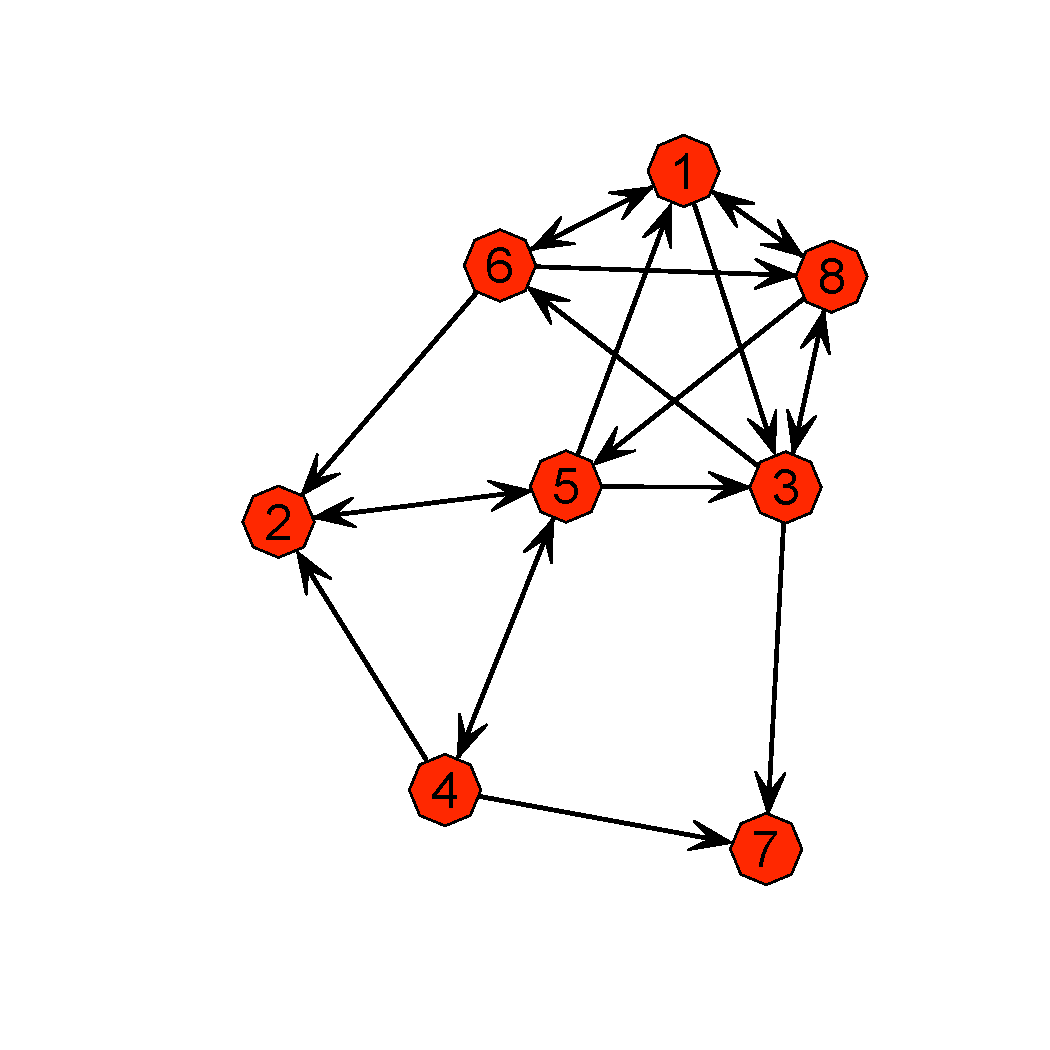
\includegraphics[height=2in, width=2in]{net8nodes.pdf}}}
$
\caption{The adjacency matrix (on left) and a corresponding graphical representation
of a directed 8-node network.  The rows of the adjacency matrix become
the out-edge lists of Figure \ref{outedgefig}.}\label{8nodeexample}
\end{figure}

\begin{figure}[htb]
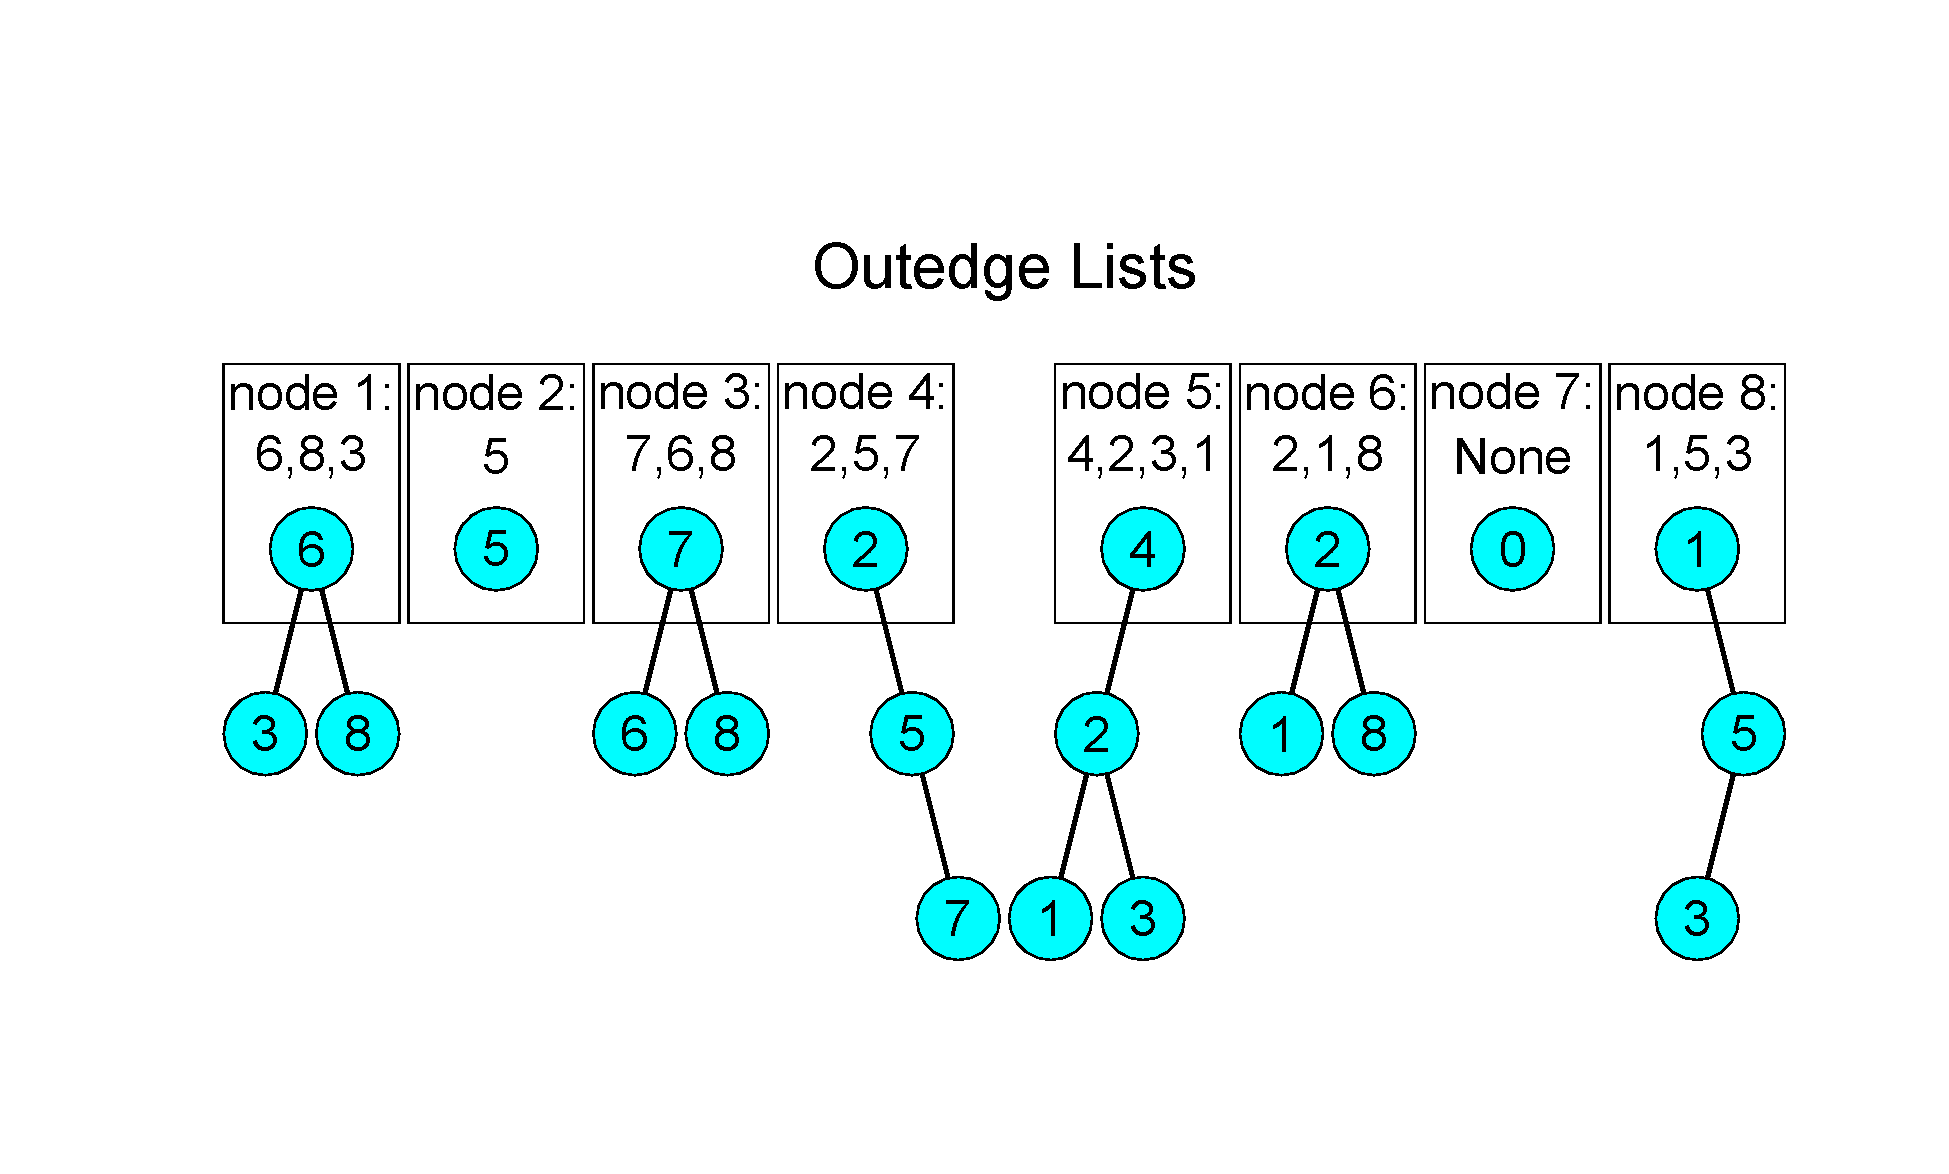
\includegraphics[height=2in, width=4in]{outedgelists.pdf}
\caption{This is the resulting internal representation of the out-edges for the network of
Figure \ref{8nodeexample}.  Each node's out-neighbors are permuted randomly 
before the binary trees are built.}\label{outedgefig}
\end{figure}

The binary tree routines, all written in the C language, are contained in the 
\code{src/edgetree.c} file in the \pkg{ergmterms} package (the \pkg{ergm} package
includes the same code).  These routines may be used to initialize or destroy
a network object, to manipulate that object by adding or deleting edges, and to
query that object to ascertain the presence of an edge.
The \code{NetworkInitialize} and \code{NetworkDestroy} functions 
are used internally by the \pkg{ergm} package to create a network object 
and destroy it when it is no longer needed by the C code.  These two functions
are not generally called by the user, though interested users may find it interesting
to look at them.  Also, the definition of the \code{Network} type, in the 
\code{src/edgetree.h} file, reveals that a network keeps updated lists of every node's
in- and out-degree in addition to the actual edges.  A user may exploit these statistics 
when writing code for various change statistics as described in Section \ref{Cside}.


\section[Writing change statistics using ergmuserterms:  The R side]%
{Writing change statistics using \pkg{ergmuserterms}:  The R side}
\label{Rside}

{\em Write this!}

\section[Writing change statistics using ergmuserterms:  The C side]%
{Writing change statistics using \pkg{ergmuserterms}:  The C side}
\label{Cside}

{\em Write this!}


EdgeTreeSearch
ToggleEdge
AddEdgeToTrees
DeleteEdgeFromTrees
EdgeTreeMinimum
EdgeTreeSuccessor





\section*{Acknowledgments}



\bibliography{v24}

\newpage

\begin{appendix}


\section[appendix]{Appendix}
\label{appendix}

\end{appendix}

\end{document}
